\chapter{Datos}


\section{Modelo de datos}


¿Qué es un modelo de datos?

Es un conjunto de tablas de datos que tienen relaciones y conexiones entre sí. Lo importante es que existan relaciones entre las diferentes tablas; relaciones de conexión entre datos como columnas o datos claves en común.

\subsection{Normalización de los datos}

Es el proceso de organización de las tablas y las columnas en una base de datos relacional para reducir la redundancia y preservar la integridad de los datos.

\begin{itemize}
    \item la eliminación de los datos para reducir el tamaño de las tablas y aumentar la velocidad y eficiencia.
    \item MInimizar las anomallías y los errores de las modificaciones de los datos.
    \item simplificación de las consultas y estructuración de la base de datos para análisis más útiles.
\end{itemize}

una buena manera de entender una base de datos normalizada es definiéndola de la siguiente manera: en una base de datos normalizada, cada tabla debe tener un \textbf{propósito único y específico}. \\

los modelos tienen generalmente dos tipos de tablas

\begin{enumerate}
    \item Tablas de datos: contiene números o valores, típicamente a nivel granular, con una columna de identificación o Id que puede ser
    \item Tablas de Vista: provee atributos descriptivos normalmente basados een texto sobre cada dimensión de la tabla. En este caso, este tipo de tablas provee mucha información sobre objetos como pueden ser ''clientes'' o ''Productos''.
\end{enumerate}

\subsection{Expresiones de análisis de datos}


Las expresiones de análisis de datos o DAX son un lenguage de fórmilas de PowerBI. Con estas fórmulas se puede hacer lo siguiente:

\begin{itemize}
    \item Añadir columnas con cálculos y mediciones al modelo, usando sintaxis intuitiva.
    \item Ir más alla de las capacidades de las formulas tradicionales, con funciones potentes y flexibles construidas específicamente para trabajar con modelos de datos relacionales.
\end{itemize}

Existen dos maneras de realizar acciones DAX: mediante creación de columnas nuevas, y mediante mediciones de un solo valor.


\subsubsection{Columnas calculadas}

Se pueden agregar columnas nuevas basadas en fórmulas a las tablas. Cosas importantes a remarcar:

\begin{enumerate}
    \item No hay referencias a celdas, todas las columnas calculadas se referencian a tablas enteras o a columnas enteras
    \item Las columnas calculadas generan valores por cada fila, los cuales son visibles dentro de las tablas en la vista de datos.
    \item Las columnas calculadas entienden el conexto de filas, lo que significa que son muy útiles para definir propiedades que estén basadas en la información de cada fila.
\end{enumerate}

Como un tip adicional y útil, use las columnas calculadas para \textbf{filtrar datos} más que para cear valores numéricos.


\paragraph*{Ejemplo}

\begin{verbatim}
    Parent = IF(Customer_Lookup[TotalChildren]>0, "Yes", "No")
\end{verbatim}

En este ejemplo se puede usar un if condicionante para agregar una columna nueva de control o de filtro.


\subsubsection{Mediciones}

En este caso son usados para generar nuevos valores calculados.

\begin{enumerate}
    \item Igual que la anterior, no hay forma de referenciar celdas aisladas; solo para tablas enteras.
    \item Estos valores no pueden ser visibles dentro de las tablas, solamente se pueden ver en elementos de visualización como cartas, o matrices.
    \item Estos cálculos siempre estarán regidos por el contexto del filtro; es decir, el valor se recalcula siempre que sea aplicado algún filtro en el elemento de visualización que se agrege o configure.
\end{enumerate}

A manera de regla general, use este tipo de cálculo cuando una única fila no puede entregarle el valor solicitado. En otras palabras, cuando necesite más de una fila.

\subsubsection{Mediciones implícitas y explícitas}

Las mediciones implícitas están en los elementos de visualización cuando uno arrastra un campo numérico a dicho elemento. Ahí es cuando se puede seleccionar el modo de agregación (suma, media, mínimo, máximo, etc).

Las mediciones explícitas, son por el contrario las que se definen de manera literal con la sintaxis de DAX

Recordando que las mediciones son evaluadas con base en el contexto de filtrado, según el filtro aplicado el resultado de la medición sera distinta. 

Por ejemplo, para la siguiente imagen, el valor sombreado es la suma del campo ´Valor´ está canlculado con base en el siguiente contexto de filtro: \texttt{IDLookup[Nombre]="Pago Obligatorio"}

\begin{figure}[H]
    \centering
    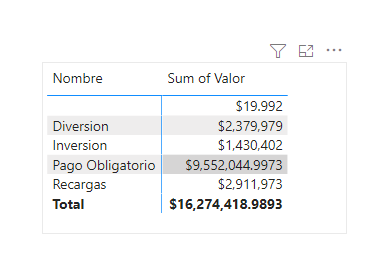
\includegraphics[scale=0.6]{Data/datafig2.png}
\end{figure}



% \begin{verbatim}
%     Overall Avg Price = CALCULATE([Avg Retail Price],ALL(AW_Products_Lookup))
% \end{verbatim}

% quita cualquier filtro de la tabla \texttt{AW\_Products\_Lookup} para tener el valor total de \texttt{Avg Retail Price} en \textbf{todas las filas}. \\

% \subsubsection*{Ejemplo de uso de filter}

% Si queremos sacar una medida de, por ejemplo, las ventas de un producto cuyo precio está por encima del promedio. \\

% \begin{verbatim}
%     High Ticket Order = CALCULATE([Total Orders], FILTER(AW_Products_Lookup,AW_Products_Lookup[ProductPrice] > [Overall Avg Price]))
% \end{verbatim}

% Aquí lo que se hace es que se pone la función filter en el filtro, el primer argumento de filter es la tabla que vamos a filtrar y el segundo argumento es la cindición de filtro.

% \begin{verbatim}
% Total Revenue_Measure = SUMX(AW_Sales,[Quantity Sold]*AW_Sales[RetailPrice])
% \end{verbatim}

% EN este caso se hace la suma total de todos los resultados de multiplicar \texttt{retailPrice} por \texttt{QuiantitySold}, como un producto punto.


% \begin{verbatim}
% Total Revenue_Measure = SUMX(AW_Sales,AW_Sales[OrderQuantity] * RELATED(AW_Products_Lookup[ProductPrice]))
% \end{verbatim}

% Esta lo que hace es traer a mi tabla de ventas, los datos relacionadosque vengan de la tabla de productos, para calcular el valor de los precios.\\

% Las siguientes son algunas fórmulas de tiempo inteligentes que pueden ser útiles: \\

% \texttt{CALCULATE(Measure, DATEYTD(Calendar[Date]) )} Si aplicamos este filtro a una medición de suma total de ingresos de ventas y ponemos en las filas los primeros días de cada mes, entonces obtenemos \\


% \texttt{YTD Revenue = CALCULATE([Total Revenue\_Measure], DATESYTD(AW\_Calendar\_Lookup[Date]))}

% Obtenemos los datos de ganancias mensualkes hasta el final de año y se inicia de nuevo en cada año

% \begin{figure}[H]
%     \centering
%     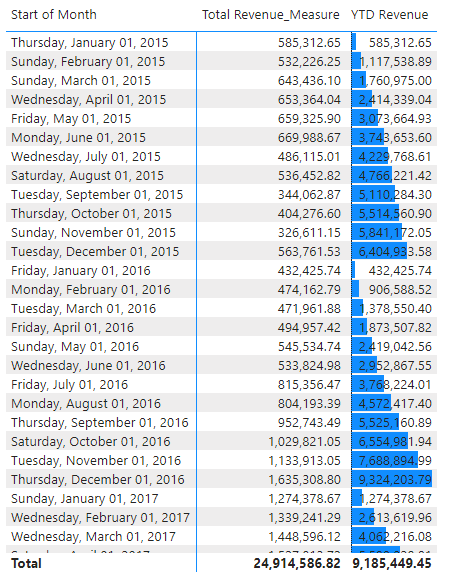
\includegraphics[scale=0.6]{Data/data1.png}
% \end{figure}



 

\texttt{CALCULATE(Measure, DATEADD(Calendar[Date], -1 , MONTH) )} Aquí la función DATEADD devuelve un rango de fechas desplazado en la cantidad y con intervalos puestos en sus argumentos \\ 
\texttt{CALCULATE(Measure, DATESINPERIOD(Calendar[Date],MAX(Calendar[Date]), -1, DAY) )} \\









\subsubsection{Sintaxis de las expresiones DAX}

Las sentencias de las expresiones se pueden separar en tres partes diferentes: nombre de la medición realizada, nombre de la función, y las referencias o argumentos de las funciones, estas pueden referirse al nombre de la tabla con su respectiva columna. También se puede estar refiriendo a una medición anteriormente definida. Como tip de utilidad, cuando nos vayamos a referir a referecias de columnas, usamos el nombre: \texttt{Table[Column]}. Y para referencias a mediciones, solo usamos el nombre de la medición: \texttt{Measure}.


Algunos operadores importantes los podemos ver en la siguiente tabla

\begin{table}[H]
    \centering
    \begin{tabular}{|c|c|c|}
        \hline
        Operador & Significado & Ejemplo\\ \hline
        + & Suma & 2 + 7 \\ \hline
        - & Resta & 5 - 3 \\ \hline
        * & Multiplicación & 2 * 6 \\ \hline
        / & División & 2 / 4 \\ \hline
        $\wedge$ & Exponente & 5 $\wedge$ 5 \\ \hline
        = & Igual a & [City] = "Boston"\\ \hline
        $>$ & Mayor & [Quantity] > 10\\ \hline
        $<$ & Menor que & [Quantity] < 10 \\ \hline
        $>=$ & Mayor o igual & [Unit\_Price] >= 2.5 \\ \hline
        $<=$ & Menor o igual & [Unit\_Price] <= 2.5 \\ \hline
        $<>$ & Diferente a & [Country] <> "Mexico" \\ \hline
        \& & Concatena dos caracteres o cadenas para formar una nueva & [City] \& "" \& [State] \\ \hline
        \& \& & AND & ([State]="MA") \& \& ([Quantity]>10) \\ \hline
        $||$ & OR & ([State]="MA") $||$ ([State]="CT") \\ \hline
        IN & Crea una condición lógica OR basada en una lista dada. & 'Store Lookup'[State] IN {"MA", "CT", "NY"} \\ \hline
    \end{tabular}
\end{table}


Las funciones también las podemos clasificar en diferentes categorías:

\begin{enumerate}
    \item Math and stats

        Tenemos aquí las funciones matemáticas de agregación más básicas y también algunas iteradoras:
        \begin{itemize}
            \item SUM
            \item AVERAGE
            \item MAX/MIN
            \item DIVIDE
            \item COUNT/COUNTA
            \item COUNTROWS
            \item DISTINCTCOUNT
            \item SUMX
            \item AVERAGEX
            \item MAXX/MINX
            \item RANKX 
            \item COUNTX
        \end{itemize}
    \item Logical functions

        Estas funciones generalmente tienen la tarea de retornar información sobre valores, con base en una expresión condicional dada. usualmente o mayoritariamente basadas en condicionales "if":
        \begin{itemize}
            \item IF
            \item IFERROR
            \item AND
            \item OR
            \item NOT
            \item SWITCH
            \item TRUE
            \item FALSE
            
        \end{itemize}
        
    \item Text functions

        Son funciones que sirven para manipular texto o formatos de control para fechas, horas o números

        \begin{itemize}
            \item CONCATENATE
            \item FORMAT
            \item LEFT/MID/RIGHT
            \item UPPEER/LOWER
            \item PROPER
            \item LEN
            \item SEARCH/FIND
            \item REPLACE
            \item REPT
            \item SUBSTITUTE
            \item TRIM
            \item UNICHAR
        \end{itemize}
    
    \item Filter functions

        Estas son funciones que están basadas en tablas relacionadas y para filtrar funciones para cálculos dinámicos.

        \begin{itemize}
            \item CALCULATE
            \item FILTER
            \item ALL
            \item ALLEXCEPT
            \item RELATED
            \item RELATEDTABLE
            \item DISTINCT
            \item VALUES 
            \item EARLIER/EARLIEST
            \item HASONEVALUE
            \item HASONEFILTER
            \item ISFILTERED
            \item USERELATIONSHIP
        \end{itemize}
        
    \item Date and time functions

            Estas son funciones especializadas en fechas y horas, así como operaciones inteligentes avanzadas
            \begin{itemize}
                \item DATEDIFF
                \item YEARFRAC
                \item YEAR/MONTH/DAY
                \item HOUR/MINUTE/SECOND
                \item TODAY/NOW
                \item WEEKDAY/WEEKNUM
                \item DATESYTD
                \item DATESQTD
                \item DATESMTD
                \item DATEADD
                \item DATESINPERIOD
            \end{itemize}
\end{enumerate}


Un par de funciones muy útiles para el manejo de las fechas son \texttt{weekday/weeknum()} y \texttt{eomonth()}. La primer función retorna el número del día de la semana de la fecha que se ponga como argumento. Por defecto, el número 1 será el día domingo, pero esto se puede cambiar mediante una opción. La segunda retorna la fecha correspondiente al último día del mes, más o menos un número especificado de meses.\\

Una de las funciones más importantes o útiles puede ser \texttt{RELATED} la cual retorna valores relacionados directamente con cada fila con base en la relación que haya con otras tablas. La sintaxis de la función es:

La función \texttt{DATEADD} Devuelve la fecha que resulta de restar o sumar la cantidad especificada en el argumento.


\begin{verbatim}
    =RELATED(ColumnName)
\end{verbatim}

el nombre de la columna es la columna de la cual se requiere extraer la información o el dato. Como tip es recomendable tratar de no crear nuevas columnas basadas en esta función, en algunas osiones esto puede ser redundante; es más recomendable usar este tipo de funciones dentro de otras como iteradores del tipo \texttt{SUMX}.



\begin{verbatim}
DATEADD(Calendar[date],-1,MONTH)
\end{verbatim}

La anterior devuelve la fecha restada en un mes

Teniendo en cuenta la tabla de gastos personal, si usamos la siguiente función:

\begin{verbatim}
YTD Gastos = CALCULATE(SUM(Gasto[Valor]), DATESYTD(Calendario_Lookup[Fecha]))
\end{verbatim}

obtenemmos la suma acumulativa de los gastos y se "renueva" en año nuevo. Observar como las barras van aumentando y el valor acumulado en el año.

\begin{figure}[H]
    \centering
    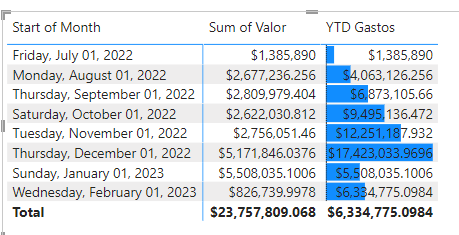
\includegraphics{Data/datafig3.png}
\end{figure}

\subsection{Parámetros 'what if'}

Este tipo de parámetros son esencialmente parámetros DAX preconfigurados que producen valores dentro de un rango dado. Este tipo de medidas pueden ser muy útiles por ejmplo para estudios de pronósticos o para estudios de posibles escenarios. para más información revisar la lección 98 del curso.


\section{SQL}



    \subsection{Conceptos}

    \subsubsection{Query}

    Es una porción de código que induce a la computadora a ejecutar una serie de operaciones y que entregará la salida requerida.


    SQL Es un lenguaje de programación declarativo no procedural. No se focaliza tanto en el procedimiento como en cuál es la tarea que se está solicitando. Su sintaxis se compone principalmente de 

    \begin{itemize}
        \item Lenguaje de definición de datos
        \item Lenguaje de manipulación de datos
        \item Lenguaje de control de datos
        \item Lenguaje de control de transacciones
    \end{itemize}

    \texttt{CREATE object\_type object\_name} \\

    \texttt{CREATE TABLE object\_name (column\_name data\_type)} \\


    \texttt{CREATE TABLE sales (purchase\_number INT data\_type)} creará una tabla llamada sales con una columna llamada purchase number del tipo entero.

    \begin{verbatim}
    ALTER TABLE sales
    ADD COLUMN date_of_purchase DATE;
    \end{verbatim}

    Se modifica la tabla agregando una columna nueva.

    \texttt{DROP TABLE customers;} borra la tabla entera \\


    \texttt{RENAME TABLE customers TO customer\_data;} cambia el nombre de la tabla. \\

    \texttt{TRUNCATE} borra los datos enteros de una tabla, pero la tabla sigue existiendo \\

    Ahora algunas palabras reservadas de DML (lenguaje de manipulación de datos)

    \texttt{SELECT .. FROM sales} selecciona lo indicado de la tabla de ventas. Se ua para extraer información de la tabla


    \texttt{INSERT INTO sales (purchase\_number, date\_of\_purchase) VALUES(1, '2017-10-11');} añade datos a la tabla

    \begin{verbatim}
    UPDATE sales 
    SET date_of_purchase = '2017-12-11'
    WHERE purchase_number = 1;
    \end{verbatim}

    Cambia directamente una entrada de la tabla


    \begin{verbatim}
    DELETE FROM sales
    WHERE
        purchase_number = 1;
    \end{verbatim}


    Sentencias para control de datos

    \begin{verbatim}
    GRANT type_permission ON database_name.table_name TO 'username'@'localhost'
    \end{verbatim}

    Otorga permisos determinados a los usuarios


    \begin{verbatim}
    REVOKE type_permission ON database_name.table_name TO 'username'@'localhost'
    \end{verbatim}

    Quita los permiso. \\

    Finalmente los comandos de control de transacciones

    \texttt{COMMIT} solamente funciona cuando se hacen cambios del tipo \texttt{INSERT}, \texttt{DELETE}, o \texttt{UPDATE}.


    \begin{verbatim}
    UPDATE customers
    SET las_name = "Johnson"
    WHERE customer_id = 4
    COMMIT;
    \end{verbatim}


    \texttt{ROLLBACK} permite devolver al estado anterior de commit

    \subsection{Pasos para crear una database y usarla}

    \begin{verbatim}
    create database if not exists Sales; 
    use Sales
    \end{verbatim}
    EL lenguaje SQL no es sensible a mayúsculas-minúsculas, ni para los nombres de los diferentes objetos, ni para las solicitudes. Esto quiere decir que \texttt{sales} y \texttt{Sales} serán iguales para SQL

    \subsection{Tipos de datos}
    Siempre es necesario especificar el tipo de datos que se insertará en cada columna de la tabla.
    \subsubsection{Cadenas de caracteres}

    Existen varios tipos de cadenas string. 

    \begin{enumerate}
        \item caracter: \texttt{CHAR}, tiene un tamaño de almacenamiento fijo y depende de qué tamaño sea declarado. \texttt{CHAR(5)} tendrá un tamaño de 5 bytes aunque el string tenga menos de 5 símbolos. 
        \item caracter variable: \texttt{VARCHAR} en este caso el tamaño de la variable no está fijo, así un \texttt{VARCHAR(5) = 'bob'} tendrá un tamaño de 3 bytes.
        \item \texttt{ENUM} Es un tipo de variable que contiene un conjunto definido total de cadenas. Por ejemplo, para el género, cuando solamente hay dos opciones para seleccionar, se puede declarar la variable \texttt{ENUM('M','F')}.
    \end{enumerate}

    Una cadena de caracteres char puede tener un tamaño máximo de 255 bytes. Un \texttt{varchar}, por su parte, puede tener un tamaño máximo de 65535 bytes. El procesamiento de las variables \textit{char} es más rápido y eficiente que el de las \texttt{varchar}, razón por la cual a veces es más conveniente declarar las primeras. \\ 

    \subsubsection{Enteros}

    La siguiente tabla resume los diferentes tipos de enteros que se pueden declarar y sus tamaños máximos así como los valores máximos que pueden tomar

    \begin{table}[H]
        \centering
        \begin{tabular}{c|c|c|c|}
        \hline
            Tipo & Tamaño & Valor mínimo (con signo/sin signo) & Valor máxumo (con signo/sin signo)  \\ \hline
            \texttt{ TINYINT }  & 1  & -128/0  & 127/255\\ \hline
            \texttt{ SMALLINT } & 2  &  -32 768/0 & 32 767/65 535\\ \hline
            \texttt{ MEDIUMINT }& 3  &  -8 388 608/0 & 8 388 607 / 16 777 215 \\ \hline
            \texttt{ INT }      & 4  & -2 147 483 648 /0  & 2 147 483 647 / 4 2094 967 295 \\ \hline
            \texttt{ BIGINT }   & 8  & -9 223 372 036 854 775 808 / 0 &  9 223 372 36 854 775 807 / 18 446 744 73 709 551 615\\ \hline
        \end{tabular}
    \end{table}

    \subsection{Variables de puntos flotantes y puntos fijos}

    En este contexto la precisión de un número se refiere a la cantidad de dígitos que hay en el mismo. Por ejemplo, \texttt{10.523} tiena una precisión de 5. Por su parte, la escala de la variable se refiere a la cantidad de dígitos que hay después del punto decimal. en el ejemplo anterior, la escala es de 3.

    Es importante saber la diferencia entre datos de punto fijo y datos de punto flotante. Los datos de punto fijo son los que representan valores exactos. Existen dos tipos de variables para los puntos fijos:

    \begin{verbatim}
    DECIMAL(5,3)
    NUMERIC
    \end{verbatim}
    Para el ejemplo \texttt{decimal(5,3)} cualquier número insertado en esta variable contendrá esta estructura. Si se inserta un \texttt{10.5} el número en realidad será \texttt{10.500}, y si se agrega un número con más decimales, entonces se redoneará para que pueda entrar en la variable, se saltará una advertencia.

    Un buen ejemplo de uso de este tipo de datos son los valores monetarios: Salarios, gastos, etc. \texttt{NUMERIC(p,s)} donde \texttt{p} representa la precisión y \texttt{s} representa la escala.


    Por su parte, los datos de coma flotante se usan para aproximar valores solamente y tiene como objetivo equilibrar el alcance y la precisión, Simplemente aproxima el valor y guarda esa aproximación. En este caso tenemos los siguientes tipos de variables para los números de coma flotante.

    \begin{verbatim}
    FLOAT
    DOUBLE
    \end{verbatim}

    \texttt{float} tiene un tamaño de 4 bytes. Es de precisión sencilla y cuenta con un máximo de 23 dígitos.  \\
    \texttt{float} tiene un tamaño de 8 bytes. Es de precisión doble y cuenta con un máximo de 53 dígitos.  \\

    \subsection{Otros tipos de datos}

    \begin{itemize}
        \item \texttt{DATE} el formato es YYYY-MM-DD. La hora no hace parte de esta representación
        \item \texttt{DATETIME} El formato es YYYY-MM-DD HH:MM:SS[.fraction]. El rango de la hora es \texttt{0 - 23:59:59.999999}
        \item \texttt{TIMESTAMP} Es el conteo en segundos desde una fecha inicial, sirve como punto de comparación entre dos fechas y establecer la diferencia en tiempo
        \item \texttt{BLOB} Significa binary large object. Se puede usar para guardar archivos de difrentes tipos: objetos binarios de gran tamaño. como fotos. 
        \item \texttt{}
    \end{itemize}


    
    \subsection{Creación de tablas}
    
    
    \begin{verbatim}
        CREATE TABLE table_name
        (
            column_1 data_type constraints,
            .
            .
            .
            column_n data_type constraints
        );
    \end{verbatim}
    
    
    Ejemplo:
    
    \begin{verbatim}
    CREATE TABLE Sales
    (
        purchase_name int not null primary key auto_increment,
        date_of_purchase date not null,
        customer_ID int,
        item_code varchar(10) not null
    );
    \end{verbatim}
    
    la sentencia \texttt{auto\_increment} asigna el número de ID a esta columna y la aunemta automáticamente. \\

    \begin{verbatim}
    CREATE TABLE Customers
    (
        customer_ID int not null primary key auto_increment,
        first_name varchar(255) not null,
        last_name varchar(255) not null,
        email_address varchar(255),
        number_of_complaints int
    );
    \end{verbatim}



    \subsection{Restricciones de SQL}

    Las restricciones son especificaciones de reglas o límites que se imponen a cada una de las columnas de la tabla. Los términos "primary key" (clave primaria) y "foreign key" (clave foránea) son fundamentales para entender cómo se relacionan las tablas entre sí y cómo se mantiene la integridad de los datos.

    \subsubsection{\texttt{primary key}}

    Una clave primaria es un campo (o conjunto de campos) que identifica de manera única cada fila en una tabla de una base de datos. Las características principales de una clave primaria son:

    \begin{enumerate}
        \item \textbf{Unicidad}: Ningún valor duplicado es permitido en una clave primaria. Cada fila debe tener un valor único para la clave primaria.
        \item \textbf{No nula}: Una clave primaria no puede tener valores nulos. Cada fila debe tener un valor para la clave primaria.
        \item \textbf{Identificación}: La clave primaria se utiliza para identificar de manera exclusiva una fila en la tabla.

    

    
    \end{enumerate}
    
    Una forma de asignar una clave primaria a una tabla es la siguiente:

    \begin{verbatim}
    CREATE TABLE Sales
    (
        purchase_number int auto_increment,
        date_of_purchase date,
        customer_ID int,
        item_code varchar(10),
    primary key (purchase_number)
    );
    \end{verbatim}
    
    
    Creamos las demás tablas con sus respectivas claves primarias:
    
    \begin{verbatim}
    create table customer
    (
        customer_id int,
        first_name varchar(255),
        last_name varchar(255),
        number_of_complaints int,
    primary key c(ustomer_id)
    );
    \end{verbatim}
    \subsubsection{\texttt{Clave foránea}}

    Una clave foránea es un campo (o conjunto de campos) en una tabla que se utiliza para referenciar la clave primaria de otra tabla. La relación entre la clave foránea y la clave primaria es lo que permite establecer relaciones entre tablas. Las características principales de una clave foránea son: 

    \begin{enumerate}
        \item \textbf{Correspondencia} con la clave primaria: Una clave foránea en una tabla corresponde a una clave primaria en otra tabla.
        \item \textbf{Integridad referencial}: La clave foránea ayuda a mantener la integridad referencial entre las tablas, asegurando que la relación entre ellas sea válida. Por ejemplo, si una fila en una tabla A hace referencia a otra fila en una tabla B, entonces la fila referenciada debe existir en la tabla B.
        \item \textbf{Valores nulos}: A diferencia de las claves primarias, las claves foráneas pueden tener valores nulos, lo que indica que no hay una relación con otra tabla.
    \end{enumerate}

    En el contexto de bases de datos relacionales, los términos "tabla padre" y "tabla hija" son fundamentales para entender cómo se estructuran y relacionan los datos. Estos conceptos están intrínsecamente vinculados a las relaciones entre tablas, en particular a través del uso de claves primarias y foráneas.

    \paragraph{Tabla Padre:} Una tabla padre, en una relación de base de datos, es aquella que tiene una clave primaria referenciada por otra tabla. La característica clave de una tabla padre es que proporciona el registro principal o la fuente de datos que otras tablas referencian. Las propiedades de una tabla padre son :

    \begin{enumerate}
        \item \textbf{Posee una Clave Primaria}: Es esencial que tenga una clave primaria, que es un identificador único para cada fila de la tabla .
        \item \textbf{Independencia}: La tabla padre puede existir en la base de datos sin la necesidad de tener una tabla hija asociada. Sus registros no dependen de la existencia de registros en otra tabla.
        \item \textbf{Fuente de Referencia}: Otras tablas (tablas hijas) hacen referencia a la tabla padre a través de sus claves foráneas, estableciendo así una relación.
    \end{enumerate}

    \paragraph{Tabla Hija:} Una tabla hija es aquella que contiene una clave foránea que hace referencia a la clave primaria de otra tabla (la tabla padre). Las características de una tabla hija son
    \begin{enumerate}
        \item \textbf{Posee una Clave Foránea}: Contiene al menos una clave foránea que establece una relación con la clave primaria de la tabla padre.
        \item \textbf{Dependencia Referencial}: La existencia de registros en la tabla hija generalmente depende de los registros en la tabla padre. Por ejemplo, no se puede insertar un registro en la tabla hija si no existe un registro correspondiente en la tabla padre, a menos que la clave foránea permita valores nulos.
        \item \textbf{Integridad Referencial}: La clave foránea asegura que las relaciones entre la tabla hija y la tabla padre sean válidas y coherentes.
    \end{enumerate}

    La forma de definir una clave foránea es 

    \begin{verbatim}
    create table sales
    (
        purchase_number int auto_increment,
        date_of_purchase date,
        customer_id int,
        item_code varchar(10),
    primary key(purchase_number),
    foreign key(customer_id) references customers(customer_id)
    );
    \end{verbatim}
    Donde la referencia se hace a la tabla que tenga esa clave como la primaria. Hay una restricción adicional llamada \texttt{on delete cascade}. Esta cláusula indica al sistema que si se elimina en la tabla padre una entrada o fila, entonces todas las entradas de la tabla hija que hagan referencia a esa clave también deberán ser borradas. 

    Se pueden modificar las características de las tablas sin necesidad de borrarlas para añadirlas nuevamente, mediante \texttt{alter}

    \begin{verbatim}
    alter table name
    add foreign key;
    drop primary key
    \end{verbatim}
    De la misma forma se puede eliminar cualquier restricción o característica.

    \subsubsection{\texttt{Clave única}}

    La restricción \verb|UNIQUE KEY|  es un tipo de restricción que se puede aplicar a una o más columnas de una tabla para asegurar que cada fila de esa columna (o combinación de columnas) tenga un valor único dentro de la tabla. Es decir, no se pueden tener dos o más filas con el mismo valor en la(s) columna(s) marcada(s) como \verb|UNIQUE|. Un ejemplo clásico de esta restricción es una columna de correos electrónicos; que no necesariamente constituye la clave principal, pero no puede ser duplicado, aunque pueden haber filas con valores en blanco en esta columna.

    Para borrar una clave única de una tabla se debe usar
    \begin{verbatim}
    drop index name;
    \end{verbatim}
    La instrucción \texttt{DROP INDEX} para eliminar una clave única \texttt{UNIQUE KEY} puede parecer inicialmente confusa, pero tiene sentido si consideramos cómo se implementan las claves únicas internamente en los sistemas de gestión de bases de datos.

    \paragraph{Implementación de Claves Únicas como Índices} Cuando se define una \texttt{UNIQUE KEY} en una tabla, la mayoría de los sistemas de bases de datos automáticamente crean un índice único para esa clave. Este índice único es lo que efectivamente garantiza la restricción de unicidad, asegurando que no se puedan insertar valores duplicados en la columna o conjunto de columnas designadas. pero ¿Por Qué Se usa \texttt{DROP INDEX}?

    \begin{enumerate}
        \item \textbf{Índices Únicos Subyacentes}: Dado que las claves únicas son implementadas internamente como índices únicos, la eliminación de una restricción de clave única implica la eliminación del índice asociado.
        \item \textbf{Consistencia con Otros Tipos de Índices:} Los RDBMS suelen tratar las claves únicas de manera similar a otros índices (como los índices normales o los índices de texto completo). Por lo tanto, se utiliza un comando común \texttt{DROP INDEX} para eliminar cualquier tipo de índice, ya sea que haya sido creado para una clave primaria, una clave única, o para optimización de consultas.
        \item \textbf{Simplificación de la Sintaxis SQL:} Utilizar un comando común para eliminar índices, independientemente de su tipo, simplifica la sintaxis del lenguaje SQL y hace que el manejo de la base de datos sea más uniforme y predecible.
    \end{enumerate}

    \subparagraph{Consideraciones Adicionales:} Es importante mencionar que la sintaxis exacta para eliminar una clave única puede variar entre diferentes sistemas de bases de datos. Algunos sistemas pueden ofrecer una sintaxis que permite eliminar directamente una clave única sin referirse explícitamente al índice. Por su parte, eliminar una clave única (y por lo tanto, el índice único asociado) debe hacerse con cuidado, ya que altera las restricciones de integridad de la tabla y puede afectar el rendimiento de las consultas.


    \subsubsection{Por defecto}

    La restricción \texttt{default} sirve para asignar un valor particular a cualquier fila de una columna; una forma de establecer un valor predeterminado para los casos en que no se especifica un valor particular al momento de añadir filas en la tabla. \texttt{number\_of\_complaints int default 0}.  Para modificar una columna y configurar su valor por defecto, se puede mediante la siguiente forma:
    \begin{verbatim}
    alter table name
    change column old_name new name new constraint;
    alter column col_name drop constraint;
    \end{verbatim}
    Las sentencias  \verb|ALTER TABLE ... CHANGE COLUMN| y \verb|ALTER TABLE ... ALTER COLUMN| son utilizadas para modificar las características de las columnas, pero tienen propósitos y comportamientos distintos. 

    \texttt{CHANGE COLUMN} se usa principalmente para cambiar el nombre de la columna, y también permite cambiar el tipo de datos de la columna y agregar o modificar restricciones.  Por su parte, \texttt{ALTER COLUMN} se usa para modificar restricciones o configuraciones de la columna ; específicamente para camiar aspectos como el valor por defecto o para modificar la capacidad de aceptar valores nulos. A diferencia de \texttt{change column}, \texttt{alter column} no se usa para cambiar el nombre de la columna o su tipo de datos.

    Hay una tercera, llamada \verb|MODIFY COLUMN|: Usado para cambiar el tipo de datos de una columna y modificar o agregar restricciones, pero sin cambiar el nombre de la columna.

    \subsubsection{\texttt{NOT NULL}}
    Esta restricción para una columna impide que una entrada nueva esté vacía; es decir, debe tener algún valor siempre. 

    \subsection{Buenas prácticas}

    Es evidente la importancia de realizar siempre un código limpio y bien entendible, organizado, cuyas secciones sean fácilmente intercambiables. Al momento de declarar nombres, asegurarse de que sean nombres cortos, con significado acorde a su función, que brinde información sobre sí mismo, que sea pronunciable. 
    La convención clásica indica que aunque SQL no distingue mayúsculas de minúsculas, es buena práctica usar mayúsculas para escribir palabras reservadas y tipos de instrucciones, y minúscula para los nombres, nunca usar espacios, y separar palabras por guión bajo.
    \subsection{Manipulación de datos}

        Una de las declaraciones más importantes en el mundo de SQL es \texttt{SELECT}. 
        \subsubsection{ \texttt{SELECT}}
        Es una declaración que permite extraer una fracción del conjunto de datos. Permite obtener datos de las tablas. Básicamente se trata de una instrucción que se usa para solicitar datos de la base de datos. La sintaxis es la siguiente:
        \begin{verbatim}
        SELECT col_1, col_2, ...
        FROM table_name;
        \end{verbatim}
        Hay una cláusula dentro de la declaración denominada \texttt{WHERE}, la cual permite establecer una condición sobre la cual se puede especificar qué parte de los datos se requiere obtener
        \begin{verbatim}
        SELECT col_1, col_2, ...
        FROM table_name
        WHERE condition;
        \end{verbatim}
        La condición puede ser cualquier valor de verdad: \texttt{WHERE first\_name = 'Denis'}. Los operadores de verdad son 

        \begin{itemize}
            \item \texttt{=}
            \item \texttt{AND}
            \item \texttt{OR}
            \item \texttt{IN}
            \item \texttt{NOT IN}
            \item \texttt{LIKE}
            \item \texttt{NOT LIKE}
            \item \texttt{BETWEEN... AND..}
            \item \texttt{EXISTS}
            \item \texttt{NOT EXISTS}
            \item \texttt{IS NULL}
            \item \texttt{IS NOT NULL}

        \end{itemize}

        Uno de interés de los anteriores es el \texttt{LIKE}, utilizando
        \begin{verbatim}
        SELECT * FROM table WHERE first_name LIKE('seb%')
        SELECT * FROM table WHERE first_name LIKE('%an')
        \end{verbatim}
        Indica una búsqueda de los nombres que empiecen por 'seb' (\texttt{'seb\%'}) o que terminen con 'an' (\texttt{\%an}). Si se usa \texttt{\%ak\%} se selecciona todas las que tengan 'ak' en cualquier parte. Si se usa por ejemplo \texttt{'Mar\_'}, entonces solo se buscará todo lo que contenga 'Mar' y \textbf{un solo caracter más}. Por parte de las fechas, SQL es capaz de realizar comparaciones entre fechas son operadores simples, por ejemplo la comparación
        \begin{verbatim} 
        hire_date > '2000-01-01'
        \end{verbatim}
        La sentencia \texttt{SELECT DISTINCT} tiene la capacidad de retornar solamente valores únicos.

        \subsubsection{Funciones agregadas}

        Se puede obtener mucha informacián de las tablas a través de las funciones de agregación 

        \begin{enumerate}
            \item \texttt{COUNT}
            \item \texttt{SUM}
            \item \texttt{MIN}
            \item \texttt{MAX}
            \item \texttt{AVG}
        \end{enumerate}

        La sintaxis es la siguiente
        \begin{verbatim}
        SELECT COUNT(col_name)
        FROM table_name
        \end{verbatim}
        Las operaciones de verdad se deben hacer directamente con las tablas:

        \begin{verbatim}
        SELECT
            COUNT(DISTINCT col_name)
        FROM
            table_name;
        \end{verbatim}
        Las funciones de gregación ignora los elementos \texttt{NULL} a menos que se le indique lo contrario. Por su parte, seleccionamos operaciones especializadas mediante la forma

        \begin{verbatim}
        SELECT
            COUNT(*)
        FROM 
            table_name
        WHERE
            col_name > 100000;
        \end{verbatim}
        \paragraph{Ordenación} Podemos ordenar el resultado con base en cualquier columna, para esto usamos \texttt{ORDER BY col\_name}:

        \begin{verbatim}
        SELECT
            *
        FROM
            table_name
        ORDER BY first_name;
        \end{verbatim} 
        Por defecto el ordenamiento es ascendente, para configurar lo contrario usamos 

        \begin{verbatim}
        SELECT
            *
        FROM
            table_name
        ORDER BY first_name DESC;
        \end{verbatim} 
        Se pueden poner varias columnas para ordenar, la primera tendreá la prioridad.

        \begin{verbatim}
        SELECT
            *
        FROM
            table_name
        ORDER BY first_name other_col ASC;
        \end{verbatim}
        \paragraph{\texttt{GROUP BY}} Todos los resultados de SQL pueden ser agrupados de acuerdo a uno o más campos específicos. La sentencia debe ser escrita inmediatamente después de la s condiciones dadas por  \texttt{WHERE} si están, y justo antes de la cláusula \texttt{ORDER BY}. El comando agrupa las filas que contienen los mismos valores en columnas especificadas en conjuntos de resumen. Estos cagrupamientos pueden usarse para realizar operaciones de agregación.
        \begin{verbatim}
        SELECT
            COUNT(first_name)
        FROM
            employees
        GROUP BY first name;
        \end{verbatim}
        Este filtro devuelve una lista con en número de veces que cada nombre se repite en toda la lista. se puede añadir el nombre para que quede más completo:
        \begin{verbatim}
        SELECT
            first_name, COUNT(first_name)
        FROM
            employees
        GROUP BY first name;
        \end{verbatim}
        De manera más compacta, escribimos un resumen de una solicitud para las tablas mediante \texttt{SELECT}:
        \begin{verbatim}
        SELECT col_name(s)
        FROM table_name
        WHERE conditions
        GROUP BY col_name(s)
        ORDER BY col_name(s)
        \end{verbatim}
        \paragraph{alias} Se usa para renombrar las columnas que extraigamos mediante alguna operación
        \begin{verbatim}
        SELECT
            first_name, COUNT(first_name) AS name_freq
        FROM
            employees
        GROUP BY first name;
        \end{verbatim}
        \paragraph{\texttt{HAVING}} Se utiliza a menudo junto con \texttt{GROUP BY} para refinar condiciones, la estructura es 
        \begin{verbatim}
        SELECT col_name(s)
        FROM table_name
        WHERE conditions
        GROUP BY col_name(s)
        HAVING conditions
        ORDER BY col_name(s)
        \end{verbatim}
        Es el equivalente al \texttt{WHERE} pero aplicado al bloque \texttt{GROUP BY}.  Un ejemplo es el siguiente

        \begin{verbatim}
        SELECT 
            first_name, COUNT(first_name) AS name_count
        FROM
            employees
        GROUP BY first_name
        HAVING COUNT(first_name) > 280
        ORDER BY first_name
        \end{verbatim}

        Es usual encontrarse en situaciones en las que no es claro la diferencia de usar \texttt{HAVING} y \texttt{WHERE}.

        La cláusula \texttt{WHERE}
        \begin{enumerate}
            \item Filtrado de Filas: \verb|WHERE| se utiliza para filtrar filas individuales antes de que se realice cualquier agrupación de datos (\verb|GROUP BY|).
            \item Operaciones en Datos Crudos: Funciona directamente sobre los datos crudos (raw data) de las tablas. Por ejemplo, puedes usar \verb|WHERE| para filtrar registros basados en condiciones específicas de las columnas de la tabla
            \item No Aplicable a Funciones de Agregación: No puedes usar \verb|WHERE| para filtrar basándote en el resultado de una función de agregación como \verb|SUM()|, \verb|AVG()|, etc.
        \end{enumerate}

        La cláusula \texttt{HAVING}
        \begin{enumerate}
            \item Filtrado de Grupos: \verb|HAVING| se utiliza para filtrar grupos creados por la cláusula \verb|GROUP BY|.
            \item Operaciones en Datos Agrupados: Funciona sobre el resultado de las funciones de agregación. Es útil cuando necesitas aplicar condiciones a un conjunto agrupado de registros.
            \item Uso Posterior a \verb|GROUP BY|: Se usa después de \verb|GROUP BY| para filtrar grupos según una condición de agregación.
        \end{enumerate}

        Un ejemplo en el que se puede usar ambos: Extraer una lista de todos los nombres que se encuentren menos que 200 veces. Los datos se deben referir a las perdonas que fueron contratadas después de primero de enero de 1999.

        \begin{verbatim}
        SELECT 
            first_name, COUNT(first_name) AS names_count
        FROM
            employees
        WHERE
            hire_date > '1999-01-01'
        GROUP BY first_name
        HAVING COUNT(first_name) < 200
        ORDER BY first_name DESC;
        \end{verbatim}
        Por último, se puede limitar el número de resultados mediante la cláusula \texttt{LIMIT}.

        \begin{verbatim}
        SELECT *
        FROM salaires
        ORDER BY salary DESC
        LIMIT 10;
        \end{verbatim}
        \subsubsection{Inserción de datos \texttt{INSERT}}

        Recordemos la sintaxis para insertar datos nuevos:
        \begin{verbatim}
        INSERT INTO table_name (col_1, ..., col_n)
        VALUES (val_1, ..., val_n)
        \end{verbatim}

        Es posible no especificar la lista de columnas que se insertan, pero en este caso es necesario siempre poner todos los valores (es decir, no omitir ninguno) y agregarlos en el mismo orden en que salen en la tabla.

        Utilizando la palabra \texttt{INTO} se pueden agregar datos de columnas de una tabla en otra, basándose en alguna condición si es necesario. Puede ser útil en la creación de tablas duplicadas para relizar algún tipo de prueba.

        \begin{verbatim}
        INSERT INTO table_2 (col_1, ..., col_n)
        SELECT col_1, ..., col_n
        FROM table_1
        WHERE condition;
        \end{verbatim}

        \subsubsection{Declaración de actualización}

            Como introducción, el concepto de Transaction Control Language (TCL) se refiere a un conjunto de instrucciones en SQL que se utilizan para manejar las transacciones en una base de datos. Una transacción es una secuencia de operaciones de base de datos que se tratan como una unidad única de trabajo. Estas operaciones deben cumplir con las propiedades ACID (Atomicidad, Consistencia, Aislamiento, Durabilidad) para asegurar la integridad y confiabilidad de la base de datos. Las instrucciones TCL permiten controlar estas transacciones para mantener la integridad de los datos y gestionar la concurrencia. Los componentes principales de TCL son:

            \begin{enumerate}
                \item \texttt{COMMIT}: Esta xomanso se utiliza para guaardar permanentemente los cambios realizasos por las transacciones en la base de datos. Una vez que se ejecuta \texttt{COMMIT}., los cambios realizados por la transacción se hacen permanentes y visibles para otrs transacciones.
                \item \texttt{ROLLBACK} ESta comando deshace todas las operaciones realizadas en la transacción actual y devuelve los datos a su estado anterior. \texttt{ROLLBACK} se utiliza en situaxiones donde se detecta un error o se necesita cancelar una transaxxión antes de hacer los cambios permanentes con \texttt{COMMIT}
            \end{enumerate}

            Evidentemene, con la declaración \texttt{UPDATE} se puese actualizar cualquier entrada de cualquier tabla de la base de datos. La sintaxis es

            \begin{verbatim}
            UPDATE table_name
            SET col_1 = val_1, ..., col_n = val_n,
            WHERE conditions
            \end{verbatim}

        \subsubsection{Declaración de borrado}

            su sintaxis es la siguiente:

            \begin{verbatim}
                DELETE FROM table_name
                WHERE conditions
            \end{verbatim}

            Es muy importante siempre tener en cuenta la relación de conexiones que existen entre dos o más tablas, pues borrar una entrada en una tabla, puede ocasionar la elomonación de sus correspondientes filas en otras tablas que estén relacionadas con ella. Esto se puede verificar en las propiedades de tabla (DDL), si existe la propiedad \texttt{ON DELETE CASCADE}. \\

            \texttt{DROP}, \texttt{TRUNCATE}, y \texttt{DELETE} son comandos en SQL utilizados para eliminar datos, pero difieren en su funcionalidad y efecto. \texttt{DROP} elimina completamente una tabla de la base de datos, borrando tanto su estructura como sus datos, y no se puede deshacer, lo que lo convierte en la opción más drástica. \texttt{TRUNCATE} también elimina todos los datos de una tabla, pero a diferencia de \texttt{DROP}, mantiene la estructura de la tabla; es más rápido que \texttt{DELETE} y reinicia cualquier contador de identidad, pero no permite condiciones y es, en general, irreversible. \texttt{DELETE}, por otro lado, es más flexible ya que permite especificar condiciones para seleccionar qué filas eliminar, mantiene la integridad de los datos y es reversible con \texttt{ROLLBACK} si se usa dentro de una transacción, aunque es más lento comparado con \texttt{TRUNCATE} para eliminar grandes cantidades de datos.

        \subsubsection{Funciones de agregación}

            Estas funciones toman la información que está contenida en varias filas de una tabla y retorna o devuelve un solo valor.

            \begin{enumerate}
                \item \textbf{COUNT}: Determina el número de filas que cumplen un criterio específico. Por ejemplo, \texttt{COUNT(*)} cuenta todas las filas en una tabla, mientras que \texttt{COUNT(column\_name)} cuenta las filas donde la columna especificada no tiene un valor NULL.
                
                \item \textbf{SUM}: Calcula la suma total de una columna numérica. Es útil para obtener el total de valores, como el total de ventas en una tabla de transacciones.
                
                \item \textbf{MIN}: Encuentra el valor mínimo en una columna dada. Esta función es empleada para identificar el valor más bajo en un conjunto de datos, como el precio más bajo de un producto.
                
                \item \textbf{MAX}: Obtiene el valor máximo en una columna. Se usa para determinar el valor más alto en un conjunto de datos, como el salario más alto entre los empleados.
                
                \item \textbf{AVG}: Calcula el valor promedio de una columna numérica. Esta función es útil para encontrar la media de valores, como el promedio de precios de productos.
                
                \item \textbf{ROUND}: Redondea un número a un número específico de decimales. Es comúnmente usada para formatear la salida de los cálculos numéricos, especialmente en los datos financieros.
                
                \item \textbf{COALESCE}: Devuelve el primer valor no NULL de una lista de expresiones. Es útil para manejar valores NULL, proporcionando una forma de definir valores predeterminados.
                
                \item \textbf{IFNULL}: Evalúa dos expresiones y devuelve la primera si no es NULL; de lo contrario, devuelve la segunda. Esta función es particularmente útil para tratar con valores NULL, permitiendo definir un valor de reemplazo cuando un campo es NULL.
            \end{enumerate}
        
            Una de las anteriores que pueden causar alguna confusión es \texttt{COALESCE}, esta función devuekve ek primer valor no nulo en una lista de argumentos. Como ejemplo, sea una tabla de empleados con columnas \texttt{ID\_empleado}, \texttt{Nombre}, \texttt{Telefono}, \texttt{Email}. En algunos casos, los empleados no han proporciondi su número de teléfono o email, por lo que estas columnas pueden contener valore nulos. Supóngase que se desea generar una lista de contactos de los empleados prefiriendo udar el teléfono, pero en caso de no estar disponible, usar el email. Es aquí donde \texttt{COALESCE} resulta útil.

            \begin{verbatim}
                SELECT
                    ID_empleado,
                    Nombre,
                    COALESCE(Telefono, Email) AS contacto,
                FROM
                    Empleados;
            \end{verbatim} 

            Esta consulta intentará primero mostrar el teléfono, pero en caso de que este valor sea nulo, entonces intentará mostrar el email. En cao de que ambos estén nulos, el resultado también será nulo. La diferencia entre \texttt{COALESCE()} y \texttt{IFNULL()} en SQL radica en su funcionalidad y flexibilidad al manejar valores nulos. Aunque ambas funciones se utilizan para lidiar con valores nulos, tienen diferencias clave en su comportamiento y uso. \texttt{COALESCE()} es más flexible y se adhiere al estándar SQL, siendo útil para múltiples argumentos, mientras que \texttt{IFNULL()} es una función más limitada y específica de MySQL, adecuada para situaciones simples de dos valores. La elección entre las dos dependerá de tus necesidades específicas y del sistema de base de datos que estés utilizando.

    \subsection{Uniones}

        Las unión es la heramienta de SQL que permite construir una relación etre las tablas. La mejor herramienta que ayuda en la búqueda de estrategias para enlazar las tablas es el esquema relacional. Como resultado, una juntura muestra un conjunto de resultados que contienen los campos derivados de dos o más tablas.

        La sintaxis para la solicitud \texttt{JOIN} es la siguiente:

        \begin{verbatim}
            SELECT
                table_1.column_name(s), table_2.column_name(s)
            FROM
                table_1
            JOIN
                table_2 ON table_1.column_name = table_2.column_name;
        \end{verbatim}

        En el primer \texttt{SELECT} se deben especificar las columinas que queremos extraer, las que queremos ver. Una forma abreviada y muy útil para este comando es:

        \begin{verbatim}
            SELECT
                t1.column_name(s), t2.column_name(s)
            FROM
                table_1 t1
            JOIN
                table_2 t2 ON t1.column_name = t2.column_name;
        \end{verbatim}

        Como consejo general, el mombre de la columna de la tabla 2 se refiere a la tabla referencia o 'Lookup'. La siguiente forma también es válida y se usa cuando se quiere primero asignar los alias de las tablas

        \begin{verbatim}
            FROM dept_manager_dup m
            INNER JOIN 
            departments_dup d ON m.dept_no = d.dept_no
        \end{verbatim}

        Anteriormente, para realizar junturas en las tabls y por ende, relaciones entre ellas, se usaba la clausula \texttt{WHERE}:

        \begin{verbatim}
            SELECT
                t1.col1, t2.col2, t3.col3
            FROM
                table1 t1
                table2 t2
            WHERE
                t1.col_name = t2.col_name
        \end{verbatim}

        Actualmente, realizar uniones de esta manera está desconsejado, pues consume más procesamiento y por ende más tiempo.

        \subsubsection{Entradas duplicadas}

        Cuando hay presencia de filas que tienen exactamente los mismos valores para todas las columnas. Generalmente, no se permiten filas duplicdas en una base de datos o tabla de datos,  es una práctica común para muchas empresas limpiar sus datos de tales ocurrencias. Sin embarago, pueden encontrarse, especialmente en datos nuevos, sin procesar o no controlados. Para manejar duplicados y evitar filas duplicadas en los resultados de las consultas, se recomienda agrupar por el campo que más difiere entre los registros. En este ejemplo, sería el número de empleado. Este enfoque apilará todas las filas que tengan el mismo número de empleado, devolviendo la salida inicial sin valores duplicados. Se resalta la importancia de esta herramienta, especialmente en bases de datos con millones de filas, donde no se debe asumir la ausencia de filas duplicadas y se aconseja acostumbrarse a agrupar las uniones por el campo que más varía entre los registros.

        \subsubsection{Función \texttt{LEFT JOIN}}

        La función \texttt{LEFT JOIN} recupera todas las filas correspondientes a la tabla derecha (la segunda tabla). Si no hay coincidencias entre las filas de la tabla izquierda y la derecha, el resultado aún uncluirá todas las filas de la tabla izquierda, pero con valores \texttt{NULL} en las columnas de la tabla derecha. Recordemos que la tabla derecha es hacia donde relacionamos (puede ser la tabla Lookup) 

        Esta función es particularmente útil cuando se necesita incluir todos los registros de de una tabla, independientemente de sis tienen una coincidencia en la otra tabla. Por ejemplo, en una consulta que une una tabla de empleados (tabla izquierda) mediante \texttt{LEFT JOIN}, se obtendrían todos los empleados incluyendo aquellos que noestén asignados a nungún departamento. Las columnas correspondientes a la taabla de departamentos mostrarían un \texttt{NULL} para  estos emopleados sin departamento asignado.

        Por su parte, tenemos la función \texttt{RIGHT JOIN}, Se trata de la función análoga a la anterior, mostrando todos los resultados de la tabla de la derecha.
        
        
        Cuando en una solicitud SQL se usan tanto \texttt{JOIN} como \texttt{WHERE}, esta última es utilizada para definir la condicioón o condiciones que determinarán cuáles van a ser los puntos de conexión entre las dos tablas

        \subsubsection{Uniones cruzadas}

        Las uniones cruzadas van a tomar los valores de cierta tabla y conectarlos con todos los valores de las tablas con las que se requiere realizar la unión. La función `CROSS JOIN` en SQL se utiliza para realizar un producto cartesiano entre dos tablas, es decir, combina cada fila de la primera tabla con cada fila de la segunda tabla. A diferencia de otros tipos de JOIN como `INNER JOIN` o `LEFT JOIN`, `CROSS JOIN` no requiere una condición de unión explícita, ya que simplemente empareja cada fila de una tabla con todas las filas de la otra tabla.

        El resultado de un `CROSS JOIN` es una tabla que contiene todas las posibles combinaciones de filas entre las dos tablas originales. Si la primera tabla tiene \( N \) filas y la segunda tabla tiene \( M \) filas, entonces el resultado del `CROSS JOIN` tendr   á \( N \times M \) filas. 
        
        Por ejemplo, si se realiza un `CROSS JOIN` entre una tabla de `Productos` y una tabla de `Vendedores`, el resultado incluirá todas las combinaciones posibles de productos y vendedores, lo cual puede ser útil para análisis que requieren considerar todas las posibles asociaciones entre dos conjuntos de datos.
        
        `CROSS JOIN` se utiliza en situaciones específicas donde se necesita explorar o analizar todas las combinaciones posibles entre dos conjuntos de datos. Sin embargo, debido a que puede generar un gran número de filas, su uso debe ser cuidadoso y bien justificado. La sintaxis sería la siguiente

        \begin{verbatim}
            SELECT 
                dm.*, d.*
            FROM
                dept_manager dm
                    CROSS JOIN
                departments d
            ORDER BY dm.emp_no , d.dept_no;
        \end{verbatim}


